\documentclass{article}
\usepackage[portuguese]{babel}
\usepackage[utf8]{inputenc}
\usepackage{amsmath, amsthm, amssymb, amsfonts}
\usepackage{listings}
\usepackage{subcaption}
\usepackage{mathtools}
\usepackage{graphicx}
\usepackage{color}
\usepackage{authblk}
\usepackage[colorlinks,citecolor=red,urlcolor=blue,bookmarks=false,hypertexnames=true]{hyperref}
\usepackage{geometry}
\usepackage{float}
\geometry{
     a4paper,
     total={170mm,257mm},
     left=20mm,
     top=20mm,
}


\newcommand{\limite}{\displaystyle\lim}
\newtheorem{teorema}{Teorema}[section]
\newtheorem{definicao}{Definição}[section]
\newtheorem{proposicao}{Proposição}[section]
\newtheorem{corolario}[teorema]{Corolário}
\newtheorem{lema}{Lema}[section]
\newtheorem{exemplo}{Exemplo}[section]
\newtheorem{theorem}{Theorem}[section]
\newtheorem{definition}{Definition}[section]
\newtheorem{collorary}[theorem]{Collorary}
\newtheorem{lemma}{Lemma}[section]
\newtheorem{proposition}{Propositon}[section]
\newtheorem{example}{Example}[section]


% Dados de identificação
\title{Notas do Curso}
\author{Patrick Oliveira}
\affil{Curso ministrado pelo Prof. Denis Fantinato, 3Q19. As notas envolvem anotações de aula e recortes de livros e artigos.} 


\begin{document}
\maketitle


Different definitions and approaches to AI.

\begin{enumerate}
    \item \textbf{Thinking Humanly}: "[The automation of] activities that we associate with human thinking, activities such as decision-making, problem solving, learning..." (Bellman, 1978)
    \item \textbf{Thinking Rationally}: "The study of the computations that make it possible to perceive, reason, and act." (Winston, 1992)
    \item \textbf{Acting Humanly}: "The art of creating machines that perform functions that require intelligence when performed by people." (Kurzweil, 1990)
    \item \textbf{Acting Rationally}: "Computational Intelligence is the study of the design of intelligent agents." (Poole \textit{et al.}, 1998)
\end{enumerate}

\section{Intelligent Agents}

An \textit{agent} is anything that can be viewed as perceiveing its \textit{environment} through \textit{sensors} and acting upon that environment through \textit{actuators}. We use the term \textit{percept} to refer to the agent's perceptual inputs at any given instant. An agent's \textit{percept sequence} is the complete history of everything the agent has ever perceived. Mathematically speaking, we say that an agent's behavior is described by the \textit{agent function} that maps any given percept sequence to an action.

The correct action is decided based on its consequences. When an agent is plunked down in an environment, it generates a sequence of actions according to the percepts it receives. This sequence causes the environment to go through a sequence of states. If the sequence is desirable, then the agent has performed well. This notion of desirability is captured by a \textit{performance measure} that evaluates any given sequence of environment variables.

What is rational at any given time depends on four things:

\begin{itemize}
    \item The performance measure that defines the criterion of success.
    \item The agent's prior knowledge of the environment.
    \item The actions that the agent can perform.
    \item The agent's percept sequence to date.
\end{itemize}

This leads to a definition of rational agent: \textit{For each possible percept sequence, a rational agent should select an action that is expected to maximize its performance measure, given the evidence provided by the percept sequence and whatever built-in knowledge the agent has.}

\section{Solving Problems By Searching}

A \textbf{problem} can be defined formally by five components:

\begin{itemize}
    \item The \textbf{initial state} that the agent starts in, e.g. \textit{In( \textbf{state} )}.
    \item A description of the possible \textbf{actions} available to the agent. Given a particular stage \textit{s}, \textit{ACTIONS(s)} returns the set of actions that can be excecuted in \textit{s}. We say that each of these actions is \textbf{applicable} in \textit{s}.
    \item A description of what each action does; the formal name for this is the \textbf{transition model}, specified by a function \textit{RESULT(s, a)} that returns the state that results from doing action \textit{a} in state \textit{a}. We also use the term \textbf{successor} to refer to any state reachable from a given state by a single action. Together, the initial state, actions, and transition model implicitly define a \textbf{state space} of the problem. The state space forms a directed network in which the nodes are states and links between nodes are actions.
    \item The \textbf{goal test}, which determines wheter a given state is a goal state.
    \item A \textbf{path cost} function that assigns a numeric cost to each path. The problem-solving agent chooses a cost function that reflects its own performance measure. 
\end{itemize}

A \textbf{solution} to a problem is an action sequence that leads from the initial state to a goal state. An \textbf{optimal solution} has the lowest path cost among all solutions.


\section{Problem Solving By Searching}

A \textbf{problem-solving agent} use \textbf{atomic} representations, states of the world that are considered as wholes, with no internal structure visible to the problem-solving algorithm. Goal-based agents that use more advanced factored or structured representations are usually called planning agents.

"Intelligent agents are supposed to maximize their performance measure." - \textit{What if an agent is composed by a different set of performance measures, competing to be minimized? How the agent would behave? The decision process would be overly complex and probably impossible to solve "analytically". We, humans, also cannot solve all the decision processes that we commit ourselves to. The constraint is time. At the end of a given time period, we make the decision that seens better under that circunstance.}

Goals help organize behavior by limiting the objectives that the agent is trying to achieve and hence the actions it needs to consider. Goal formulation, based on the current situation and the agent's performance measure, is the first step in problem solving.

We will consider a goal to be a set of world states - exactly those states in which the goal is satisfied. The agent's task is to find out how to act so that it reaches a goal state. Problem formulation is the proess of deciding what actions and states to consider, given a goal.


\noindent \textit{There can be an agent that learns the map of the environment where it is in? The map can be about the set of possible world states.}

If the agent does not have additional information about the problem that it is trying to solve, i.e., if the environment is unknown, then it is has no choice but to try one of the actions at random. But the agent can have a map; the point of a map is to provide the agent with inormation about the states it might get itself into and the actions it can take. The agent can use this information to consider subsequente stages. In general, an agent with several immediate options of unknown value can decide what to do by first examining future actions that eventually lead to states of known value.

The environment can be 

\begin{itemize}
    \item \textbf{observable:} The agent always knows the current state.
    \item \textbf{discrete:} so at any given state there are only finitely many actions to choose from. \textit{What would be the mathematical consequences if we consider an enumerable set of possible actions? Or a uncountable set of possible actions? There can be a logical formulation of a decision process? Can i prove theorems about that?}
    \item \textbf{known:} the agent knows which states are reached by each action.
    \item \textbf{deterministic:} each action has exactly one outcome.
\end{itemize}

Under these assumptions, the solution to any problem is a fixed sequence of actions. The process of looking for a sequence of actions that reaches the goal is called a \textbf{search}. A search algorithm takes a problem as input and returns a \textbf{solution} in the form of an action sequence. Once a solution is found, the actions it recommends can be carried out. This is called the \textbf{execution} phase. While the agent is executing the solution sequence it ignores its percepts when choosing an action because it knows in advance what they will be. Control theorists call this an open-loop system, because ignoring the percepts breaks the loop between agent and environment.

\subsubsection{Well-defined problems and solutions}

A problem can be defined formally by five components:

\begin{itemize}
    \item The \textbf{initial state} that the agent starts in.
    \item A description of the possible \textbf{actions} available to the agent. Given a particular state s, Actions(s) returns the set of actions that can be executed in s. We say that each of these actions is applicable in s.
    \item A description of what each action does; the formal name for this is the \textbf{transition model}, specified by a function Result(s, a) that returns the state that results from doing action a in state s. Together, the initial state, actions, and transition model implicitly define the \textbf{state space} of the problem - the set of all states reachable from the initial state by any sequence of actions. The state space forms a directed network or graph in which the nodes are states and the links between nodes are actions. A \textbf{path} in the state space is a sequence of states connected by a sequence of actions.
    \item The \textbf{goal test}, which determines whether a given state is a goal state. SOmetimes the goal is specified by an abstract property rather than an explicitly enumerated set of states.
    \item A \textbf{path cost} function that assigns a numeric cost to each path.
\end{itemize}

\subsection{Searching for Solutions}

A solution is an action sequence, so search algorithms work by considering various possible action sequences. The possible action sequences starting at the initial state form a \textbf{search tree} with the initial state at the root. The branches are actions and the \textbf{nodes} correspond to states in the state space of the problem.

The first step is to test whether this is a goal stage. Then we need to consider taking various actions. We do this by expanding the current state; that is, applying each legal action to the current state, thereby generating a new set of states. In this case, we add three branches from the parent node, leading to new childs nodes. The set of all leaf nodes avaialble for expansion at any given point is called the \textbf{frontier}.

The frontier separates the state-space graph into the explored region and the unexplored region, so that every path from the initial state to an unexplored state has to pass through a state in the frontier. As every step moves a state from the frontier, we see that the algorithm is systematically examining the states in the state space, one by one, until it finds a solution.

The process of expanding ndoes on the frontier continues until either solution is found or there are no more states to expand. Search algorithms all share this basic structure; they vary primarily according to how they choose which state to expand next - the so-called search strategy.

A repeated state in the search tree is generated by a loopy path. Loopy paths means that the complete search tree is infinite because there is no limit to how often one can traverse a loop. Loopy paths are a special case of the more general concept of redundant paths, which exist whenever there is more than one way to get from one state to another. In some cases, it is possible to define the problem itself so as to eliminate redundant paths. In other cases, redundant paths are unavoidable. This includes all problems where the actions are reversible. 

The way to avoid exploring redundant paths is to remember where one has been. To do this, we augment the Tree-Search algorithm with a data structure called the explored set (also known as the closed list), which remembers every expanded node.

\subsubsection{Infrastructure for search algorithms}

For each node n of the tree, we have a structure that contains four components:

\begin{itemize}
    \item \textbf{n.State.}
    \item \textbf{n.Parent.}
    \item \textbf{n.Action.}
    \item \textbf{n.Path-cost.}
\end{itemize}

\begin{figure}
     \center
     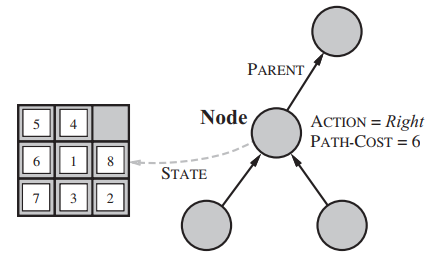
\includegraphics[scale = 1]{node_ds.png}
     \caption{Nodes are the data structures from which the search tree is constructed.}
     \label{fig:node_ds}
\end{figure}

The frontier needs to be stored in such a way that the search algorithm can easily choose the next node to expand according to its preferred strategy. The appropriate data structure for this is a queue.

\subsubsection{Measuring problem-solving performance}

We can evaluate an algorithm's performance in four ways:

\begin{itemize}
    \item Completeness: Is the algorithm guaranteed to find a solution when there is one?
    \item Optimality: Does the strategy find the optimal solution?
    \item How long does it take to find a solution?
    \item How much memory is needed to perform the search?
\end{itemize}

In AI, the graph is often represented implicitly by the initial state, actions, and transition model and is frequently infinite. For these reasons, complexity is expressed in terms of three quantities: b, the branching factor or maximum number of successors of any node; d, the depth of the shallowest goal node. Time is often measured in terms of the number of nodes generated during the search, and space in terms of the maximum number of nodes stored in memory.

To assess the effectiveness of a search algorithm, we can consider just the search cost, or we can use the total cost, which combines the search cost and the path cost of the solution found.

\subsection{Uninformed Search Strategies}

\subsubsection{Breadth-first search}

Breadth-first search is an instance of the general graph-search algorithm in which the shallowest unexpanded node is chosen for expansion. This is achieved very simply by using a FIFO queue for the frontier. Thus, new nodes (which are always deeper than their parents) go to the back of the queue, and old nodes, which are shallower than the new nodes, get expanded first. There is one slight tweak on the general graph-search algorithm, which is that the goal test is applied to each node when it is generated rather than when it is selected for expansion. The algorithm is complete, if the shallowest goal node is at some finite depth d, breadth-first search will eventually find it after generating all shallower nodes. Now, the shallowest goal node is not necessarily the optimal one.

\begin{lstlisting}[caption = Breadth-first search on a graph]
function Breadth-First-Search(problem) returns a solution, or failure

    node = a node with "State = problem.Initial-State, Path-Cost = 0"
    if problem.Goal-Test(node.State) then return Solution(node)
    frontier = a FIFO queue with node as the only element
    explored = an empty set
    loop do
        if Empty?(frontier) then return failure
        node = Pop(frontier)
        add node.State to explored
        for each action in problem.Actions(node.State) do 
            child = Child-Node(problem, node, action)
            if child.State is not in explored or frontier then 
                if problem.Goal-Test(child.State) then return Solution(child)
                frontier = Insert(child, frontier)
\end{lstlisting}

\subsubsection{Uniform-cost search}

When all step costs are equal, breadth-first search is optimal because it always expands the shallowest unexpanded node. By a simple extension, we can find an algorithm that is optimal with any step-cost function. Instead of expanding the shallowest node, uniform-cost search expands the node n with the lowest path cost g(n). This is done by storing the frontier as a priority queue ordered by g. The goal test is applied to a node when it is selected for expansion, to avoid selecting a solution that was generated first but that is suboptimal.

\begin{lstlisting}[caption = Uniform-cost search on a graph.]
function Uniform-Cost-Search(problem) returns a solution, or failure

    node = a node with "State = problem.Initial.State, Path-Cost = 0"
    frontier = a priority queue ordered by Path-Cost, with node as the only element
    explored = an empty set 
    loop do 
        if Empty?(frontier) then return failure 
        node = Pop(frontier)
        if problem.Goal-Test(node.State) then return Solution(node)
        add node.State to explored 
        for each action in problem.Actions(node.State) do 
            child = Child-Node(problem, node, action)
            if child.State is not in explored or frontier then 
                frontier = Insert(child, frontier)
            else if child.State is in frontier with higher Path-Cost then 
                replace that frontier node with child 
\end{lstlisting}

Uniform-cost search is optimal in general. First, we observe that whenever uniform-cost search selects a node n for expansion, the optimal path to that node has been found. Then, because step costs are nonnegative, paths never get shorter as nodes are added. These two facts together imply that uniform-cost search expands nodes in order of their optimal path cost. Hence, the first goal node selected for expansion must be the optimal solution. 

\subsubsection{Depth-first search}

Depth-first search always expands the deepest node in the current frontier of the search tree. The search proceeds immediately to the deepets level of the search tree, where the nodes have no successors. It uses a LIFO queue.

The properties of depth-first search depend strongly on whether the graph-search or tree-search version is used. The graph-search version, which avoids repeated states and redundant paths, is complete in finite state spaces because it will eventually expand every node. The tree-search version, on the other hand, is not complete. Depth-first tree search can be modified at no extra memory cost so that it checks new states against those on the path from the root to the current node; this avoids infinite loops in finite state spaces but does not avoid the proliferation of redundant paths.

\subsubsection{Depth-limited search}

The embarassing failure of depth-first search in infinite state spaces can be alleviated by supplying depth-first search with a predetermined depth limit $ l $. This approach is called depth-limited search. The depth limit solves the infinite-path problem. Unfortunately, it also introduces an additional source of incompleteness if we choose $ l < d $. Depth-limited search will also be nonoptimal if we choose $ l > d $. Depth limits can be based on knowledge of the problem.

\begin{lstlisting}
function Depth-Limited-Search(problem, limit) returns a solution, or failure/cutoff
    return Recursive-DLS(Make-Node(problem.Initial-State), problem, limit)

function Recursive-DLS(node, problem, limit) returns a solution, or failure/cutoff
    if problem.Goal-Test(node.State) then return Solution(node)
    else if limit = 0 then return cutoff
    else
        cutoff_occurred? = false 
        for each action in problem.Actions(node.State) do 
            child = Child-Node(problem, node, action)
            result = Recursive-DLS(child, problem, limit - 1)
            if result = cutoff then cutoff_occurred? = true 
            else if result != failure then return result 
        if cutoff_occurred? then return cutoff else return failure
\end{lstlisting}

\subsubsection{Iterative deepening depth-first search}

Iteratie deepening search (or iterative deepening depth-first search) is a general strategy, often used in combination with depth-first tree search, that finds the best depth limit. It does this by gradually increasing the limit until a goal is found.

Iterative deepening search may seem wasteful because states are generated multiple times. It turns out this is not too costly. The reason is taht in a search tree with the same (or nearly the same) branching factor at each level, most of the nodes are in the bottom level, so it does not matter much that the upper levels are generated multiple times.

\begin{lstlisting}
function Iterative-Deepening-Search(problem) returns a solution, or failure
    For depth = 0 to inf do 
        result = Depth-Limited-Search(problem, depth)
        if result != cutoff then result result
\end{lstlisting}

It's possible to use a hybrid approach that runs breadth-first search until almost all the avaialble memory is consumed, and then runs iterative deepening from all the nodes in the frontier. In general, iterative deepening is the preferred uninformed search method when the search space is alrge and the depth of the solution is not known. 

\subsubsection{Bidirectional search}

The idea behind bidirectional search is to run two simultaneous searches - one forward from the initial state and the other backward from the goal - hoping that the two searches meet in the middle. The motivation is that $ b^{d/2} + b^{d/2} $ is much less than $ b^d $.

Bidirectional search is implemented by replacing the goal test with a check to see whether the frontiers of the two searches intersect; if they do, a solution has been found. The check can be done when each node is generated or selected for expansion and, with a hash table, will take constant time. How to search backward? Let the predecessors of a state x be all those states that have x as a sucessor. Bidirectional search requires a method for computing predecessors. When all the actions in the state are reversible, the predecessors of x are just its successors. Other cases may not be like that. 

\begin{figure}
     \center
     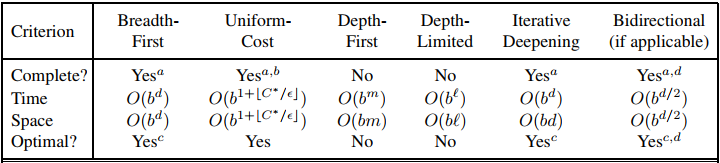
\includegraphics[scale = 0.8]{search_comparison.png}
     \caption{Evaluation of tree-search strategies.}
     \label{fig:search_comparison}
\end{figure}

\subsection{Informed Search Strategies}

The general approach we consider is called best-first search. Best-first search is an instance of the general Tree-Search or Graph-Search algorithm in which a node is selected for expansion based on an evaluation function, $ f(n) $. Most best-first algorithms include as a component of $ f $ a heuristic function, denoted $ h(n) $:

$$ h(n) = \text{ estimated cost of the cheapest path from the state at node n to a goal state.} $$

\subsubsection{Greedy best-first search}

Greedy best-first search tries to expand the node that is closest to the goal, on the grounds that this is likely to lead to a solution quickly. Thus, it evaluates nodes by using just the heuristic function; that is, $ f(n) = h(n) $. The algorithm is called "greedy" because at each step it tries to get as close to the goal as it can.

Greedy best-first tree teach is incomplete even in a finite state space, because of closed loops. The graph search version is complete in finite spaces, but not in infinite ones.

\subsubsection{A* search: Minimizing the total estimated solution cost}

The A* search evaluates nodes by combining $ g(n) $, the cost to reach the node, and $ h(n) $, the cost to get from the node to the goal:

$$ f(n) = g(n) + h(n) $$

Provided that the heuristic function $ h(n) $ satisfies certain conditions, A* search is both complete and optimal.

The first condition we require for optimality is that $ h(n) $ be an \textbf{admissable heuristic}. An admissable heuristic is one that \textit{never overestimates} the cost to reach the goal. Admissable heuristics are by nature optimistic because they think the cost of solving the problem is less than it actually is.

A second, slightly stronger condition stronger condition called \textbf{consistency} (or sometimes \textbf{monoticity}) is required only for applications of A* to graph search. A heuristic h(n) is consistent if, for every node n and every successor n' of n generated by any action a, the estimated cost of reaching the goal from n is no greater than the step cost of getting to n' plus the estimated cost of reaching the goal from n':

$$ h(n) \leq c(n, a, n') + h(n') $$

For an admissible heuristic, the inequality makes perfect sense: if there were a route from $ n $ to $ G_{n} $ via $ n' $ that whas chepaer than $ h(n) $, that would violate the property that $ h(n) $ is a lower bound on the cost to reach $ G_n $.

\textbf{Every consistent heuristic is also admissible:} By contradiction.

A* has the following properties: \textit{the tree-search version of A* is optimal if h(n) is admissible, while the graph-search version is optimal if h(n) is consistent}. Lets consider the second claim.

If h(n) is consistent, then the vlaues of f(n) along any path are nondecreasing. Suppose n' is a successor of n; then $ g(n') = g(n) + c(n, a, n') $ for some action a, and we have

$$ f(n') = g(n') + h(n') = g(n) + c(n, a, n') + h(n') \geq g(n) + h(n) = f(n) $$

The next step is to prove that whenever A* selects a node n for expansion, the optimal path to that node has heen found. Were this not the case, there would have to be another frontier node n' on the optimal path from the start node to n; because f is nondecreasing along any path, n' would have lower f-cost than n and would have been selected first.

From the two preceding observations, it follows that the sequence of nodes expanded by A* using Graph-Search is in nondecreasing order of f(n). Hence, the first goal node selected for expansion must be an optimal solution because f is the true cost for goal nodes (which have = 0) and all later goal nodes will be at least as expensive.

The fact that f-costs are nondecreasing along any path also means that we can draw countours in the state space, just like the contours in a topographic map. With uniform-cost search (A* search using h(n) = 0), the bands will be "circular" around the start state. With more accurate heuristics, the bands will stretch toward the goal state and become more narrowly focused around the optimal path. 

If C* is the cost of the optimal solution path, then we can say the following:

\begin{itemize}
    \item A* expands all nodes with f(n) < C*
    \item A* might then expand some of the nodes on the "goal countor" before selecting a goal node
\end{itemize}

Completeness (if there is a solution for the problem it will be found) requires that there be only finitely many nodes with cost less than or equal to C* (with A*, if there is a solution to be found, it will be the optimal one), a condition that is true if all step costs exceed some finite $\varepsilon$ and if b is finite. The condition on the step cost guarantees that the algorithm wont stuck in a loop with cost zero, and the second guarantees that the number of branches will be finite.

A* is \textbf{optimally efficient} for any given consistent heuristic. That is, no other optimal algorithm is guaranteed to expand fewer nodes than A*. This is because any algrorithm that does not expand all nodes with f(n) < C* runs the risk of missing the optimal solution.

There is the difficulty that, for most problems, the number of states within the goal contour search space is still exponential in the length of the solution. 

\subsubsection{Memory-bounded heuristic search}

The simplest way to reduce memory requirements for A* is to adapt the idea of iterative deepening to the heuristic search context, resulting in the iterative-deepening A* (IDA*) algorithm. The main difference between IDA* and standard iterative deepening is that the cutoff used is the f-cost (g+h) rather than the depth; at each iteration, the cutoff is the smallest f-cost of any node that exceeded the cutoff on the previous iteration. 

\begin{lslisting}[caption = Recursive best-first search.]
    function Recursive-Best-First-Search(problem) returns a solution, or failure
        return RBFS(problem, Make-Node(problem.Initial-State), inf)

    function RBFS(problem, node, f_limit) returns a solution, or failure and a new f-cost limit
        if problem.Goal-Test(node.State) then return Solution(node)
        successors = []
        for each action in problem.Actions(node.State) do 
            add Child-Node(problem, node, action) into successors 
        if successors is empty then return faiilure, inf 
        for each s in successors do 
            s.f = max(s.g + s.h, node.f)
        loop do 
            best = the lowest f-value node in successors 
            if best.f > f_limit then return failure, best.f 
            alternative = the second-lowest f-value among successors 
            result, best.f = RBFS(problem, best, min(f_limit, alternative))
            if result != failure then return result
\end{lslisting}

Recursive best-first search (RBFS) is a simple recursive algorithm that attempts to mimic the operation of standard best-first search, but using only linear space. Its structure is similar to that of a recursive depth-first search, but rather than continuing indefinitely down the current path, it uses the f_limit variable to keep track of the f-value of the best alternative path available from any ancestor of the current node. If the current node exceeds this limit, the recursion unwinds back to the alternative path. As the reursion unwinds, RBFS replaces the f-value of each node along the path with a backed-up value - the best f-value of its children. 

Like A* tree search, RBFS is an optimal algorithm if the heuristic function h(n) is admissible. 

IDA* and RBFS suffer from using too little memory. Between iterations, IDA* retains only a single number: the current f-cost limit. Because they forget most of what they have done, both algorithms may end up reexpanding the same states many times over. It seems sensible, therefore, to use all available memory. Two algorithms taht do this are MA* (memory-bounded A*) and SMA* (simplified MA*). SMA* proceeds just like A*, expanding the best leaf until memory is full. SMA* always drops the worst leaft node - the one with the highest f-value. LIKE RBFS, SMA* then backs up the value of the forgotten node to its parent. If all the descendants of a node n are forgotten, then we will not know which way to go from n, but we will still have an ideia of how worthwhile it is to go anywhere from n.

What if all the leaf nodes have the same f-value? SMA* expands the newest best leaf and deletes the oldest worst leaf. If the leaf is not a goal node, then even if it is on an optimal solution path, that solution is not reachable with the available memory.

SMA* is complete if there is any reachable solution. It is optimal if any optimal solution is reachable. On very hard problems, it will often be the case that SMA* is forced to switch back and forth continually among many candidate solution paths, only a small subset of which can fit in memory.


\end{document}
